\documentclass[acmlarge]{acmart}

\usepackage[
    type={CC},           % your choice
    modifier={by},       % your choice
    version={4.0},       % your choice
]{doclicense}            % your choice, see \doclicenseThis below

\settopmatter{printacmref=false}
\fancyfoot{}

\makeatletter
\def\@formatdoi#1{}
\def\@permissionCodeOne{miniKanren.org/workshop}
\def\@copyrightpermission{\doclicenseThis} % your choice of text
\def\@copyrightowner{Copyright held by the author(s).} % your choice
\makeatother

\copyrightyear{2019}
\setcopyright{rightsretained}

% Metadata Information
\acmJournal{PACMPL}
% \acmVolume{1}
% \acmNumber{ICFP} % CONF = POPL or ICFP or OOPSLA
\acmYear{2019}
\acmMonth{8}
\acmArticle{4}
% \acmDOI{} % \acmDOI{10.1145/nnnnnnn.nnnnnnn}

% \startPage{1}

\usepackage{booktabs} 
\usepackage{listings}
\usepackage[justification=centering]{caption}
\usepackage{subcaption}
% \usepackage{cite}
\usepackage{amssymb}
\usepackage{amsmath}
\usepackage{amsthm}
\usepackage{mathtools}
\usepackage{xspace}
\usepackage{bussproofs}
\usepackage{tikz}
\usepackage{float}
\usepackage{graphicx}
\usepackage{array}
\usepackage{tabularx}
\usepackage{collcell}
\usepackage[ruled]{algorithm2e} 

% \SetAlFnt{\small}
% \SetAlCapFnt{\small}
% \SetAlCapNameFnt{\small}
% \SetAlCapHSkip{0pt}
% \IncMargin{-\parindent}

% Paper history
% \received{February 2007}
% \received{March 2009}
% \received[accepted]{June 2009}

\bibliographystyle{ACM-Reference-Format}

\citestyle{acmauthoryear}

\newcommand{\rulehskip}{\hskip 1.5em}
\newcommand{\rulevspace}{\vspace{1em}}

\newcommand{\pvfill}{\pause\vfill}

% \mathchardef\mhyphen="2D

\theoremstyle{definition}

\newtheorem{example}{Example}[section]
\newtheorem{definition}{Definition}
\newtheorem{lemma}{Lemma}
\newtheorem{remark}{Remark}
\newtheorem{theorem}{Theorem}

\newenvironment{subproof}[1][\proofname]{%
  \renewcommand{\qedsymbol}{$\blacksquare$}%
  \begin{proof}[#1]%
}{%
  \end{proof}%
}

% \newtheorem{prop}{Proposition}

%% \counterwithin{lemma}{section}

\newcommand{\textdef}[1]{\textit{#1}}

\newcommand{\imm}{{\textrm IMM}~}

% inline code 
\newcommand{\code}[1]{\texttt{#1}}

% tuple with angle brackets
\newcommand{\tup}[1]{\langle #1 \rangle}

% semantics brackets
\newcommand{\sem}[1]{\llbracket #1 \rrbracket}

% equality by definition
\newcommand{\defeq}{\triangleq}

% function arrow
\newcommand{\fun}{\rightarrow}

% partial function arrow
\newcommand{\pfun}{\rightharpoonup}

% some math sets
\newcommand{\N}{{\mathbb{N}}}
\newcommand{\Q}{{\mathbb{Q}}}

% domain/codomain notation
\newcommand{\dom}[1]{\textit{dom}{({#1})}}
\newcommand{\codom}[1]{\textit{codom}{({#1})}}

\newcommand{\isground}[1]{\textit{is\_ground}({#1})}

\newcommand{\mgu}{\textit{mgu}}

\newcommand{\vars}[1]{\textit{Vars}({#1})}

\newcommand{\sapp}[2]{{#2}{#1}}
\newcommand{\subs}{\sqsubseteq}

% some logical notation
%\newcommand{\implies}{{\Rightarrow}}
%\newcommand{\iff}{{\Leftrightarrow}}

% check-mark and cross-mark
\newcommand{\cmark}{\text{\color{green!60!black}\ding{51}}}
\newcommand{\xmark}{\text{\color{red!60!black}\ding{55}}}

%% axiom labels

\newcounter{mylabelcounter}

\makeatletter
\newcommand{\labelAxiom}[2]{%
\hfill{\normalfont\textsc{(#1)}}\refstepcounter{mylabelcounter}
\immediate\write\@auxout{%
  \string\newlabel{#2}{{\unexpanded{\normalfont\textsc{#1}}}{\thepage}{{\unexpanded{\normalfont\textsc{#1}}}}{mylabelcounter.\number\value{mylabelcounter}}{}}
}%
}
\makeatother

%% warning

\colorlet{colorWARNING}{yellow!90!black}

% \newcommand{\warning}[1]{{\color{colorWARNING}\texttt{WARNING}}: #1}
% \newcommand{\app}[1]{{\color{blue}\textbf{ANTON: #1}}}
% \newcommand{\note}[1]{{\color{cyan}\textbf{EVG: #1}}}

\newcommand\ExecScaleFactor{1}

\newcommand{\todo}[1]{{\color{red}\textbf{TODO: #1}}}

%% OCanren's listings

\lstdefinelanguage{ocanren}{
    keywords={fresh, let, in, match, with, when, class, type,
    object, method, of, rec, repeat, until, while, not, do, done, as, val, inherit,
    new, module, sig, deriving, datatype, struct, if, then, else, open, private, virtual, include, success, failure,
    true, false},
    sensitive=true,
    commentstyle=\small\itshape\ttfamily,
    identifierstyle=\ttfamily,
    keywordstyle=\bfseries,
    basewidth={0.5em,0.5em},
    columns=fixed,
    fontadjust=true,
    abovecaptionskip=\bigskipamount,
    literate={->}{{$\to$}}3 {===}{{$\equiv$}}1 {=/=}{{$\not\equiv$}}1 {|>}{{$\triangleright$}}3  {/\\}{{$\wedge$}}2 {\\/}{{$\vee$}}2 {^}{{$\uparrow$}}1 {'}{{$^\prime$}}1 {~}{{$\neg$}}1 {=>}{{$\Rightarrow$}}2, 
    morecomment=[s]{(*}{*)}
}

\lstset{
    mathescape=true,
    %basicstyle=\small,
    commentstyle=\scriptsize\rmfamily,
    language=ocanren,
    captionpos=b,
    % escapeinside={(*}{*)},
}

\newcolumntype{H}{>{\collectcell\lstinline}l<{\endcollectcell}}

% Document starts
\begin{document}

% Title portion
\title{Constructive Negation for MiniKanren} 

\author{Evgenii Moiseenko}
%\authornote{with author2 note}          %% \authornote is optional;
                                        %% can be repeated if necessary
\orcid{nnnn-nnnn-nnnn-nnnn}             %% \orcid is optional
\affiliation{
  %\position{Position2a}
  %\department{}             %% \department is recommended
  \institution{Saint Petersburg State University}           %% \institution is required
  %\streetaddress{Street2a Address2a}
  \city{Saint Petersburg}
  %\state{Russia}
  %$postcode{Post-Code2a}
  %\country{Russia}                   %% \country is recommended
}
\email{e.moiseenko@2012.spbu.ru}         %% \email is recommended
\affiliation{
  %\position{Position2b}
  %\department{Department2b}             %% \department is recommended
  \institution{JetBrains Research}           %% \institution is required
  %\streetaddress{Street3b Address2b}
  %\city{City2b}
  %\state{State2b}
  %\postcode{Post-Code2b}
  %\country{Country2b}                   %% \country is recommended
  \country{Russia}
}
%\email{first2.last2@inst2b.org}         %% \email is recommended

\begin{abstract}

We present an extension of \textsc{MiniKanren} with the negation operator
based on the method of \emph{constructive negation}.
The idea of this method is to constructively 
build a stream of answers for the negated goal
by collecting and negating individual answers
to the positive version of the goal.
As we demonstrate on the series of examples 
constructive negation suits to pure logical nature of \textsc{MiniKanren}:  
the relations involving the negation operator 
still can be ``run'' in various directions.

\end{abstract}


%
% The code below should be generated by the tool at
% http://dl.acm.org/ccs.cfm
% Please copy and paste the code instead of the example below. 
%
\begin{CCSXML}
  <ccs2012>
    <concept>
      <concept_id>10011007.10011006.10011008.10011009.10011012</concept_id>
      <concept_desc>Software and its engineering~Functional languages</concept_desc>
      <concept_significance>500</concept_significance>
    </concept>
    <concept>
      <concept_id>10011007.10011006.10011008.10011009.10011015</concept_id>
      <concept_desc>Software and its engineering~Constraint and logic languages</concept_desc>
      <concept_significance>500</concept_significance>
    </concept>
  </ccs2012>
\end{CCSXML}

\ccsdesc[500]{Software and its engineering~Functional languages}
\ccsdesc[500]{Software and its engineering~Constraint and logic languages}

\keywords{relational programming, constructive negation, OCanren}

\maketitle
\thispagestyle{empty}

% !TEX TS-program = pdflatex
% !TeX spellcheck = en_US
% !TEX root = main.tex


\section{Introduction}
\label{sec:intro}


One of distinguishable features of \miniKanren{} is the fact that it is a family of languages:
many languages may host different \miniKanren{} implementations.
For example, \faster{}\footnote{\url{https://github.com/michaelballantyne/faster-minikanren} (access date: \DTMdate{2024-06-06})} for \Scheme{} and \Racket{}, \CoreLogic{} for \textsc{Closure}, \OCanren{}~\cite{OCanren} for \OCaml{}, \Klogic{}~\cite{Klogic2023} for \Kotlin{} and others.
The users of these DSLs may want to compare expressive power of various flavor of miniKanren, specifics due to host language, and performance implications of choosing a different host language.


The straightforward solution is to rewrite a number of significant benchmarks for many implementation, as it done for other languages\footnote{\url{https://benchmarksgame-team.pages.debian.net/benchmarksgame/index.html} (access date: \DTMdate{2024-06-06})}.
Doing it manually is time consuming and error prone.
Due to low-level nature of relational programs, it is easy to make spelling mistakes, for example accidentally write wrong identifier in unification arguments.
(We did many of mistakes of this kind while porting programs from \OCanren{} to \Klogic{}.) Moreover, \miniKanren{} doesn't pardon relational programs that solve the same task: it was reported, that the order of conjuncts significantly affects~\cite{scheduling2022} performance even if the search does the same unifications.

The differences between host languages also complicate porting relational code.
For example, \Kotlin{} doesn't support currying and partial applications comparatively to \OCaml{}, and sometimes full $\eta$-expansion is needed.
Also, porting from dynamically typed languages like \Scheme{} to statically typed ones like \OCaml{} could be uneasy for newcomers to statically typed languages.
This porting could be not straightforward:
basic data representations in \OCaml{}/\Klogic{} (algebraic data types and classes with subclasses~--- sum types) is different from \Scheme{} (lists, i.e. arbitrary length tuples~--- product types).
This fact in some cases requires special constraints~\cite{Wildcards2023} to level the expressivity, and in other cases (like relational interpreters) allows to get rid of \emph{absento/symbolo} constraints.

Things could get even more complicated where we want to port larger projects which are using functional/relational approach where relational parts are intermixed with straightforward programming.
The developer is obliged to know relational approach, the original host general purpose language and to have experience  with a new host language.

In this paper we describe current status of our converter from relational \OCanren{} to \Klogic{} and \miniKanren{} in \Scheme{}.
At the moment only relational subset of \OCanren{} is supported, we don't support whole \OCaml{} language.
In next section we describe technical aspects of our approach and currently supported features.
In section \ref{sec:interpreter} we discuss transformation in relational interpreter~\cite{Untagged} from \OCanren{} to \Scheme{} and peculiarities of autogenerated implementation.



\section{Motivating Examples}

\label{sec:motivation}

In this section we give further motivation 
for adding the negation into relational programming.
We present several examples of how the negation can be used.

\subsection{Relational If-then-else}

\label{sec:ifte}

In the Prolog one can simulate the conditional if-then-else
operator using so-called \emph{soft cut}~\cite{naish1995pruning}.
The behavior of the soft cut \lstinline{c $\rightarrow^*$ t ; e}
can be described as follows:

\begin{itemize}
  \item if the goal \lstinline{c} succeeds 
        (i.e. produces at least one answer) then
        the result of \lstinline{c $\rightarrow^*$ t ; e}
        is equivalent to \lstinline{c /\ t};
  \item if the goal \lstinline{c} fails 
        (i.e. produces no answers at all) then
        the result of \lstinline{c $\rightarrow^*$ t ; e}
        is equivalent to \lstinline{e}.
\end{itemize}

The soft cut is an example of a non-relational feature.
Such features usually do not compose well
in the sense that they are sensitive to the 
order in which they appear in a program.
For example, consider the goal 
\lstinline{(c $\rightarrow^*$ t ; e) /\ g},
and assume that \lstinline{c /\ g} always fails
regardless of the order of conjuncts.
Then if \lstinline{c} succeeds the result 
of the above goal will be equivalent to 
\lstinline{c /\ t /\ g} and thus it will fail.
Suppose we reorder the conjuncts as follows:
\lstinline{g /\ (c $\rightarrow^*$ t ; e)}.
Now the goal \lstinline{c}, when executed after \lstinline{g}, 
certainly fails, and thus the result 
of the whole goal will be equivalent to
\lstinline{g /\ e} which does not fails necessarily.
One can see that the simple reordering 
of subgoals in the program can lead to the different results.

With the help of constructive negation
if-then-else can be simply expressed as follows:

\begin{minipage}[h]{\textwidth}
\begin{lstlisting}[
  % caption={Logical if-then-else},
  label={lst:ifte},
  escapeinside={(*}{*)},
]
let ifte c t e = 
  (c /\ t) \/ (~ c /\ e)
\end{lstlisting}
\end{minipage}

The behavior of if-then-else defined in this way
subsumes the behavior of the soft cut.
That is, every answer to the query \lstinline{run (c $\rightarrow^*$ t ; e)}
is also an answer to the query \lstinline{run (ifte c t e)}.
Moreover, \lstinline{ifte} is not sensitive to the order
of subgoals in the program.

\subsection{Classical Implication and Universal Quantification}

\label{sec:impl-univ}

With the negation added to the language, one can easily express other 
connectives of the classical first-order logic,
namely the implication and universal quantification\footnote{
It is easy to see that \lstinline[mathescape]{c => t} 
is equivalent to \lstinline{ifte c t succ}},
using the well-known equivalences.

\begin{minipage}[h]{\textwidth}
\begin{lstlisting}[
  % caption={Implication and universal quantification},
  label={lst:impl-univ},
  escapeinside={(*}{*)},
]
let (=>) : goal -> goal -> goal = 
  fun g$_1$ g$_2$ ->  ~ g$_1$ \/ (g$_1$ /\ g$_2$)

let forall : ('a -> goal) -> goal = 
  fun g -> ~ fresh (x) (~ g x)
\end{lstlisting}
\end{minipage}

% There are at least two common interpretations of universal quantification.
% Under the \emph{intentional} interpretation we assume that 
% $\forall x. P(X)$ is true if $P(c)$ is true for 
% an arbitrary choice of some constant $c$.
% Under the \emph{extensional} interpretation 
% $\forall x. P(X)$ is true if $P(t)$ is true for every $t$.
% The \lstinline{forall} presented above implements 
% the extensional universal quantification.

However, we should make a few remarks here.
It is well known that the search implemented 
in conventional \textsc{MiniKanren} is complete, 
meaning that every answer to an arbitrary query 
will be found eventually. 
In the presence of constructive negation 
(and thus implication and universal quantification defined through negation)
the search becomes incomplete as we will later see.
Moreover, constructive negation is computationally heavy
and thus the double usage of it,
as in the definition of \lstinline{forall},
can be inefficient in some cases.

Despite all this trouble we have found that 
the above definitions are still useful.
Some of the previous \textsc{MiniKanren} implementations 
introduced \emph{eigen} variables,
adopted from $\lambda$Prolog~\cite{miller2012programming}.
Eigen variables act as a universally quantified variables.
Yet, to the best of our knowledge,
there is no sound implementation of eigen variables
with the support of disequality constraints.
We observed that our implementation 
of universal quantifications through double negation 
works nicely with disequalities 
(we give some examples in the Section~\ref{sec:evaluation}).
 
\subsection{Graph Unreachability Problem}

One of the classical examples of negation application 
in logic programming is a problem of checking whether 
one node of the graph is unreachable 
from the another~\cite{przymusinski1989constructive}.
The code on Listing~\ref{lst:unreach}
defines binary relation \lstinline{edge},
which binds pairs of nodes in graph, 
connected by some edge,
and binary relation \lstinline{reachable},
which is nothing more than a 
transitive closure of the \lstinline{edge} relation.
Then the relation \lstinline{unreachable}
is simply negation of \lstinline{reachable}.

\begin{minipage}[h]{\textwidth}
\begin{lstlisting}[
  caption={Unreachability in a graph},
  label={lst:unreach},
  escapeinside={(*}{*)},
]
let edge x y = 
  (x, y) === ('a', 'b') \/
  (x, y) === ('b', 'a') \/
  (x, y) === ('b', 'c') \/
  (x, y) === ('c', 'd') 

let reachable x y = 
  x === y \/
  fresh (z) (
    edge x z /\ reachable z y
  )

let unreachable x y = 
  ~(reachable x y)
\end{lstlisting}
\end{minipage}

Given this definition the query \lstinline{run unreachable 'c' 'a'} will succeed.
A knowledgeable reader might notice that 
constructive negation is not necessary in this case 
because negation as failure will deliver the same result.
But the query \lstinline{run unreachable 'c' q} will fail under
negation as failure because of the free variable \lstinline{q} which 
will appear under the negation.
However constructive negation will succeed 
delivering the constraint \lstinline{q =/= 'd'}.

\subsection{Unreachability in Labeled Transition Systems}

One can consider a special kind of graphs --- 
\emph{labeled transition systems}~\cite{baier2008principles}.
Labeled transition system is defined by a set of states $S$,
a set of labels $L$ and a ternary transition relation $R \subseteq S \times L \times S$.
By existential quantification over labels one can then obtain a binary relation. 
Taking its transitive closure gives the reachability relation.
The negation of the reachability relation can be used 
to check that some state $s'$ is not reachable from the initial state $s$.
The Listing~\ref{lst:lts} shows an encoding of an
abstract labeled transition system in \textsc{OCanren}.

Labeled transition systems are often used to 
describe the behavior of imperative languages.
Although the naive encoding of transition relation in \textsc{OCanren}
with simple enumeration of reachable states is often
not tractable for checking reachability (or unreachability) in 
huge state spaces arising in practical imperative programs,
it still can be used, for example, for the task of 
prototyping the semantics of such languages.

\begin{minipage}[htp]{\textwidth}
\begin{lstlisting}[
  caption={Unreachability in a labeled transition system},
  label={lst:lts},
  escapeinside={(*}{*)},
]
module type LTS = sig
  type state
  type label

  val transition : state -> label -> state -> goal
end

module LTSExt (T : LTS) = struct

  let reachable : T.state -> T.state -> goal = 
    fun s s'' -> 
      s === s'' 
      \/
      fresh (l s') (
        T.transition s l s' /\
        reachable s' s''
      )

  let unreachable : T.state -> T.state -> goal = 
    fun s s' -> 
      ~(reachable s s')
end

\end{lstlisting}
\end{minipage}
% !TEX TS-program = pdflatex
% !TeX spellcheck = en_US
% !TEX root = main.tex

\section{Implementation and Evaluation}

\begin{figure*}[t]
\begin{verbnobox}[\fontsize{10pt}{10pt}\selectfont]
ordered main_group (
  Label "Type" describes TextEdit "Any" {width=200}
  Label "Owner" describes TextEdit "Anyone" {width=200}
  Label "Has the words" describes TextEdit "Enter words found in the file" {
   width = 400
  }
  Label "Item name" describes
    TextEdit "Enter a term that matches part of the file name" {
      width = 400
    }
  (Label "Location" describes
    (TextEdit "Anywhere" { width = 200 }) dominates
    ordered location_checkboxes (
      Label "In trash"  describes CheckBox in_trash_checkbox
      Label "Starred"   describes CheckBox starred_checkbox
      Label "Encrypted" describes CheckBox encrypted
    )
  )
  Label "Date modified" describes  TextEdit "Any time" {width=200}
  Label "Approvals" describes
    ordered approvals_checkboxes (
      Label "Awaiting my approval" describes CheckBox awaiting_checkbox
      Label "Requested by me" describes CheckBox requestred_checkbox
  )
  Label "Shared to" describes
    TextEdit "Enter a name or email address..." {width=400}
  Label "Follow-ups" describes TextEdit "---" {width=200, height=35}
)
Button "Search" approves^ main_group
Button "Reset" cancels^ main_group
\end{verbnobox}
\caption{Google Drive Search Settings Dialog Structure Description}
\label{gd_structure}
\end{figure*}

\begin{figure*}[t]
    \begin{subfigure}[t]{.45\textwidth}
        \vspace{-15em}
        \begin{minipage}{4cm}
        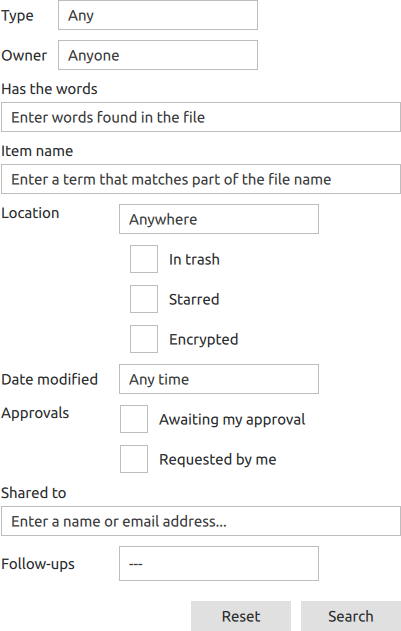
\includegraphics[scale=0.5]{google-drive-search-setting-output2.png}
        \end{minipage}
        \caption{If label describes controls which are ``too long'', then place them vertically}
    \end{subfigure}\hspace{1cm}
    \begin{subfigure}[t]{.45\textwidth}
      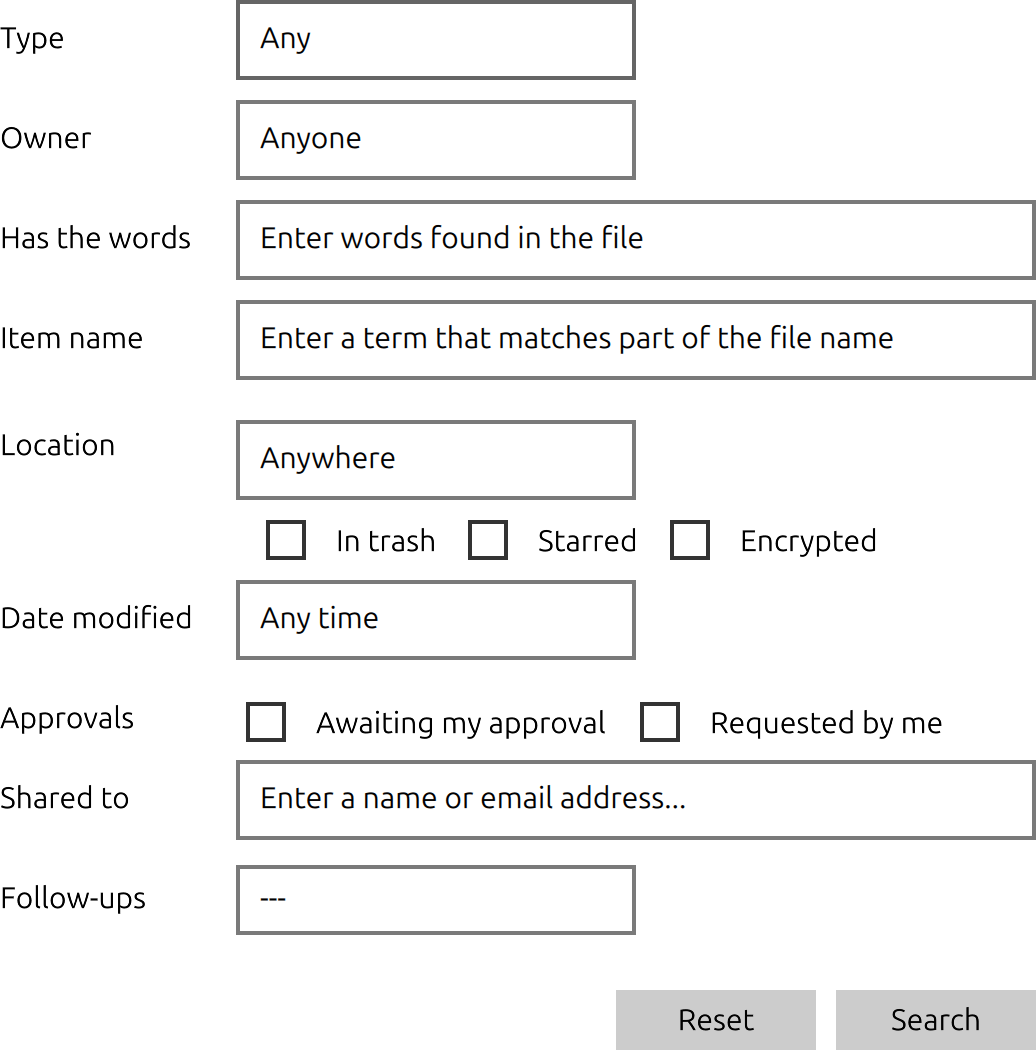
\includegraphics[scale=0.5]{google-drive-search-setting-output3.png}
      %\vskip17.5mm
      \caption{The same, but the constant for ``too long'' was decreased}
    \end{subfigure}
    \caption{Google Drive Search Settings Dialog Layouts}
    \label{fig:QMLtwoGuidelines}
\end{figure*}

\newcommand{\OCaml}{\textsc{OCaml}\xspace}
\newcommand{\OCanren}{\textsc{OCanren}\xspace}
\newcommand{\noCanren}{\textsc{noCanren}\xspace}
\newcommand{\Zthree}{\textsc{Z3}\xspace}
\newcommand{\JSOO}{\textsc{Js\_of\_ocaml}\xspace}

%In this section we describe technical details of our prototype implementation and show a few examples of layout synthesis for specific GUI structures.

The prototype of our synthesizer is developed as a \mbox{client}/server application using web technologies\footnote{The implementation is available online
for review: \url{https://genui.utbot.org}, username: ``public-user'', password: ``1jWMz2oWWmQW40hHSPZb'', no quotes.
%In case it doesn't work try \url{https://se.math.spbu.ru/genui}.
Generated design will be shown below specification field.}.
On the client side we use \textsc{HTML5} for rendering and \OCaml
compiled to \textsc{JavaScript} via \JSOO~\cite{JSOO} for a client-server interaction. The server side is a native \OCaml application equipped with \OCanren and \Zthree.
%An initial attempt was to build a serverless prototype but, first, we observed that \JSOO runs as twice as slower than the native \OCaml even for simple cases, and,
%second, we found making \Zthree to run in a web-browser a burden.

In order to provide end-users a way to represent GUI structures and guidelines we developed two textual DSLs. In addition in our implementation
the expressivity of guidelines description was a little bit extended~--- for example, we actually allow the rules to be equipped with custom constraints, there are
some extra constructs to express the guidelines for table-like layouts, etc. None of these extensions compromise the approach we
described in the previous sections and all of them can rather easily be taken into account. We also parameterized our system with
a set of constants which describe the common properties of the environment (for example, the size of the pane to place the synthesized layout in).
An example of structure description for Google Drive search settings dialog is shown in Fig.~\ref{gd_structure}.
The textual representation of guidelines, however, is too lengthy to show.


\begin{comment}
The flowchart of server-side application architecture is shown in Fig.~\ref{server-flowchart}. Dotted blocks denote the input data (structure,
guideline and environment descriptions), blocks with solid thin borders~--- \OCaml non-relational components, blocks with solid thick borders~---
relational components written in \OCanren. Thin arrows show the data transfer between components, and the thick one~--- the execution
of generated from inputs relational program. By ``run$^*$'' we denote the execution of relational components which return all the answers for the problem
they solve. The last two steps (integer linear inequations generation and \Zthree execution) are performed for each synthesized hypercube.

\begin{figure}[h]
%  \centering
  \includegraphics[scale=0.5]{server-flowchart.eps}   % if it fails to compile install 'texlive-font-utils'
  \caption{The architecture of server-side application}
  \label{server-flowchart}
\end{figure}
\end{comment}

\begin{comment}
\begin{figure*}
  \begin{tabular}{m{7.5cm}|m{10.5cm}}
    \begin{lstlisting}[basicstyle=\small]
| Descr (l, cb), Type (cb, CheckBox)
  => Hor (cb, l)

| Ord (x, y) => Vert (x, y), Halign (x, y)

| Sub (x, y) => Vert (x, y), Indent (x, y)

\end{lstlisting} & \multirow{3}{*}{
\begin{tabular}{c}
	\parbox{9cm}{There are no such explicit rules in the guideline, but these basic cases implicitly follow from the others.}
\end{tabular}}\\
\hline
\begin{lstlisting}[basicstyle=\small]
| Descr (X, Y), not (Type (Y, Checkbox)),
  width (Y) <= K
  => Hor (X, Y)
\end{lstlisting} & \multirow{2}{*}{
\begin{tabular}{c}
	{ \parbox{9.5cm}{
					\vspace{-1em}
If an input box is long, and the horizontal space is limited, place the label above the box. Otherwise, always put the label and the box on the same line.
	}}\\
  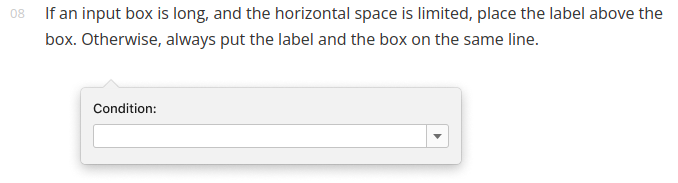
\includegraphics[scale=0.3]{jbg-08.png} \\
%  \includegraphics[scale=0.3]{jbg-08-new.png} \\
  {\parbox{9.5cm}{\textit{By the second rule variable $X$ is a label with text ``Condition'' and variable $Y$ is a drop-down list.}}}
\end{tabular}}\\
\begin{lstlisting}[basicstyle=\small]
| Descr (X, Y), not (Type (Y, Checkbox)),
  width (Y) > K
  => Vert (X, Y), Halign (X, Y)
\end{lstlisting} & \\ \\
\hline
\begin{lstlisting}[basicstyle=\small]
| Ord (v1, v2),
  Comp (v1, c1), not (Type (c1, CheckBox)),
  Comp (v2, c2), not (Type (c2, CheckBox)),
  Descr (l1, c1), Descr (l2, c2),
  width c1 $\leqslant\!$ 100, width c2 $\leqslant\!$ 100
  => (
  | width l1 $\!\geqslant\!$ width l2, width l1 $\leqslant\!$ width l2 $\cdot$ 2
  | width l1 $\!<\!$ width l2, width l2 $\leqslant\!$ width l1 $\cdot$ 2
    => Halign (c1, c2))
\end{lstlisting} &
\begin{tabular}{c}
{\parbox{9.5cm}{
%		\vspace{-4em}
	By default, put input controls with labels of similar length on different lines and align their input boxes on the left side.
}}\\
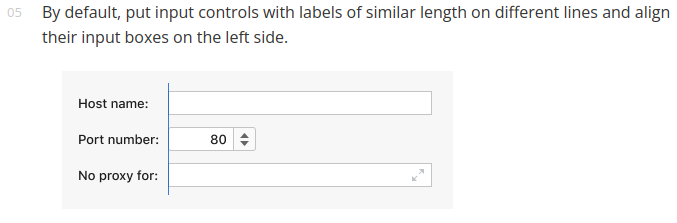
\includegraphics[scale=0.3]{jbg-05.png} \\
%\includegraphics[scale=0.2]{jbg-05-new.png} \\
{\parbox{9.5cm}{\textit{The rule applied twice. In the first case virtual control $C$ contains the top textbox $Y$ and virtual control $C^\prime$ contains the middle textbox $Y^\prime$. The textbox $Y$ is described by the top label $X$ and the textbox $Y^\prime$ is described by the middle label $X^\prime$. The second case is similar for middle and bottom controls.}}}
\end{tabular}
\\
\\
\hline
\begin{lstlisting}[basicstyle=\small]
| Ord (v1, mid),
  Ord (mid, v2),
  Comp (v1, c1), not (Type (c1, CheckBox)),
  Comp (v2, c2), not (Type (c2, CheckBox)),
  Descr (l1, c1), Descr (l2, c2),
  width c1 $\leqslant\!$ 100, width c2 $\leqslant\!$ 100
  => (
  | width l1 $\!\geqslant\!$ width l2, width l1 $\leqslant\!$ width l2 $\cdot$ 2
  | width l1 $\!<\!$ width l2, width l2 $\leqslant\!$ width l1 $\cdot$ 2
    => Halign (c1, c2))
\end{lstlisting} &
\begin{tabular}{c}
{\parbox{9.5cm}{
%		\vspace{-4em}
	If there are two input controls with labels of similar length that are separated from each other by a single control, align their input boxes on the left side.
}}\\
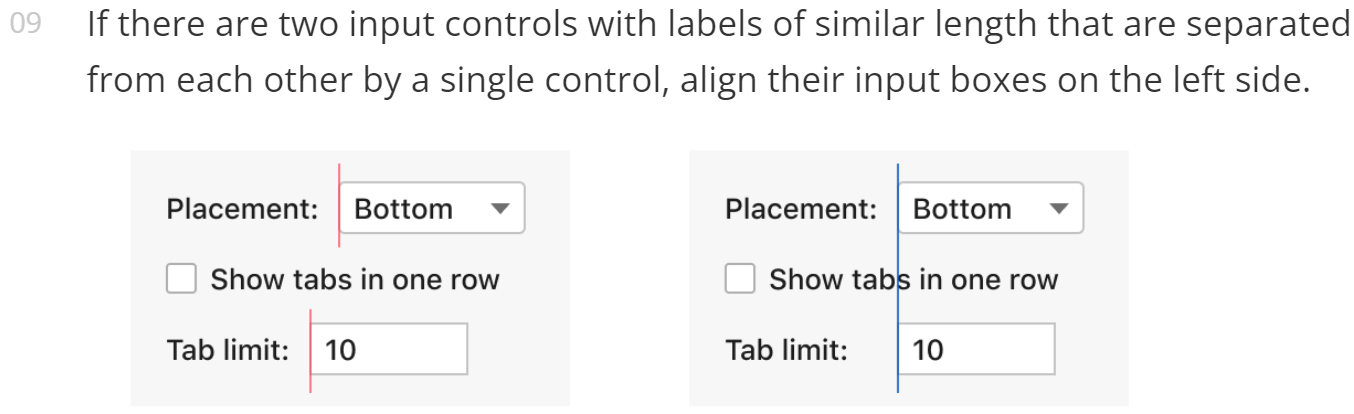
\includegraphics[scale=0.3]{jbg-09.png} \\
%\includegraphics[scale=0.4]{jbg-09-new.png} \\
{\parbox{9.5cm}{\textit{By the rule virtual control $C$ contains the top textbox $Y$ and virtual control $C^{\prime}$ contains the bottom textbox $Y^\prime$. There is a virtual control $Y^{\prime\prime}$ containing the checkbox between them. Labels $X$ and $X^\prime$ describe textboxes $Y$ and $Y^\prime$.}}}
\end{tabular}
  \end{tabular}
  \caption{Examples of GUI guidelines specification (based on informal JetBrains guidelines rules 05, 08 and 09)}
  \label{guidelines-example}
\end{figure*}
\end{comment}

%\subsection{Client Side}
%A web page is essentially a text area for the user input of structure information in the syntax similar to that in Fig.~\ref{fig:evaluation},
%and a space for rendering results. The client-server interaction runs in several phases. The client sends structure information to the server and receives possibly many layouts. After that it sends the %layouts to the server one by one and receives the exact coordinates of the UI elements in the structure. The layouts which were successfully evaluated with \Zthree are being rendered in the end.

%\subsection{Server Side}
%The server side is implemented in \OCaml with assistance of \OCanren\footnote{
%\href{https://github.com/PLTools/OCanren}{https://github.com/PLTools/OCanren}
%\url{https://github.com/PLTools/OCanren}
%}~\cite{Zthree}, \noCanren\footnote{\url{https://github.com/Lozov-Petr/noCanren}}~\cite{lozov2017typed}
% and \Zthree~\cite{Zthree}. It could be separated into two parts: synthesis of a layout and evaluation of absolute coordinates.

%The synthesis of a layout is implemented mostly in functional style with assistance of \noCanren, which translates a dialect of \textsc{ML} to \OCanren. The exception is a
%confirmation check (described in Section~\ref{sec:synthesizing}) which is easier to implement in relational style because it applies non-deterministically many guideline rules.
%Encoding of the guideline rules themselves in \OCanren is error-prone because of inversion requirement. We implemented an embedded DSL for \OCaml for these guidelines
%which performs an inversion at compile time.

%We could name two drawbacks in our current implementation.  For now we have a limited amount of identifiers for UI elements (named by letters from A to J on
%Figure \ref{fig:evaluation}) which allows to represent our binary hypercube finitely, but
%reduces the expressivity of input structure definition. In future it shall be easily fixed because all possible structure definitions have a finite number
%of elements. Another drawback of our binary hypercube is an ability to encode nonsensical layouts (for example, one element subordinates another and vice versa).
%Right now these layouts are filtered out during the generation of absolute coordinates, but ideally we want them to be non-representable using type definitions of our synthesizer.

%The second part of server implementation is the calculation of absolute coordinates with assistance from \Zthree. This stage filters out problematical layouts and performs much
%faster than our relational synthesis. But we linked \OCaml and \Zthree to a single executable anyway  to avoid paying any costs  for inter process communication.

To evaluate our prototype in the context of the real world GUI framework we implemented a renderer based on Qt/QML. On Fig.~\ref{fig:QMLtwoGuidelines} you can see two layouts of the
Google Drive search settings dialog structure rendered  w.r.t. two slightly different versions of JetBrains GUI guidelines~\cite{JBG} using QtQuick Controls\footnote{\url{https://doc.qt.io/qt-5/qtquick-controls2-qmlmodule.html}} and Material Design theme. The guideline says that if a text edit is ``too long'', one has to put it below the label.
On the bottom layout the
factor describing the informal notion of ``being too long'' was increased. The synthesis of each layout took 5 seconds.

A few more examples are shown in Fig.~\ref{fig:evaluation}.


%As an example of GUI synthesis we show the results of synthesis for a few GUI structures w.r.t. JetBrains GUI guidelines~\cite{JBG}.
%%\footnote{https://jetbrains.github.io/ui/principles/layout}.
%The results are shown in Fig.~\ref{fig:evaluation}. As one can see, a proper layout was synthesized in each case, and the synthesis time for each was no more than 5 seconds.

\begin{figure*}
    \begin{tabular}{m{95mm}m{5cm}}
      \begin{lstlisting}[basicstyle=\small]
  ordered (
    Label "Short label"     describes TextEdit "Text 1"
    Label "Loooooong label" describes TextEdit "Text 2"
  )
      \end{lstlisting} &
      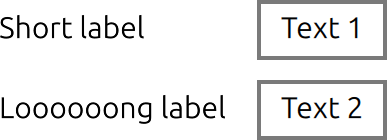
\includegraphics[scale=0.5]{Example1-Qt-QML.png} \\
      \hline\\
      \begin{lstlisting}[basicstyle=\small]
  ordered (
    Label "Looooong label" describes TextEdit "Text 1"
    Label "Medium label"   describes TextEdit "Text 2"
    Label "Short"          describes TextEdit "Text 3"
  )
      \end{lstlisting} &
      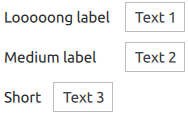
\includegraphics[scale=0.5]{Example2-Qt-QML.png} \\
      \hline
      \begin{lstlisting}[basicstyle=\small]
  ordered (
    Label "Short label"     describes TextEdit "Text 1"
    Label "Check box label" describes CheckBox _
    Label "Looooong label"  describes TextEdit "Text 2"
  )
      \end{lstlisting} &
      \vspace{1em}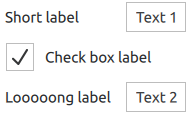
\includegraphics[scale=0.5]{Example4-Qt-QML.png} \\
      \hline\\
      \begin{lstlisting}[basicstyle=\small]
  ordered (
    Label "L 1"     describes CheckBox _
    Label "Lab 2"   describes CheckBox _
    Label "Label 3" describes CheckBox _
    Label "Label 4" describes CheckBox _
    Label "L 5"     describes CheckBox _
    Label "Lab 6"   describes CheckBox _
  )
      \end{lstlisting} &
      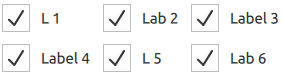
\includegraphics[scale=0.5]{Example5-Qt-QML.png} \\
    \end{tabular}
    \caption{Examples of structures (left) and synthesized layouts (right)\\
      w.r.t. JetBrains guidelines}
    \label{fig:evaluation}
  \end{figure*}

\section{Evaluation}

\label{sec:evaluation}

In this section, we present an evaluation of 
implemented constructive negation on a series of examples.

\subsection{If-then-else}

Using relational if-then-else operator, 
presented in section~\ref{sec:ifte},
we have implemented several 
higher-order relations over lists, namely 
\lstinline{find} (Listing~\ref{lst:eval-find}), 
\lstinline{remove}\footnote{Note, this implementation 
differs from the one in Section~\ref{sec:intro}, but 
it is easy to see that these two are semantically equivalent.} (Listing~\ref{lst:eval-remove}) 
and \lstinline{filter} (Listing~\ref{lst:eval-filter}).
These relations are almost identical (syntactically) to their
functional implementations.
We have tested that these relations can be run
in various directions and produce the expected results.
For example, the goal \lstinline{filter p q q}
with the predicate \lstinline{p} equal to

\begin{lstlisting}
  fun l -> fresh (x) (l === [x])
\end{lstlisting}

stating that the given list should be a singleton list,
starts to generate all singleton lists.
Vice versa, the goal \lstinline{filter p q []} 
with that same \lstinline{p} generates 
all lists, constrained to be not a singleton list.

Listings~\ref{lst:eval-p}-\ref{lst:eval-filter-queries} give 
more concrete examples of queries to these relations.
In the listing the syntax \lstinline{run n q g}
means running a goal \lstinline{g} with 
the free variable \lstinline{q}
taking the first \lstinline{n} answers (``\lstinline{*}'' denotes all answers).
After the sign $\leadsto$ the result of the query is given.
The result \lstinline{fail} means that the query has failed.
The result \lstinline[mathescape]|succ {{a$_1$}; ... {a$_n$}} |
means that the query has succeeded delivering $n$ answers.
Each answer represents a set of constraint on free variables.
Constraints are of two forms: equality constraints, e.g. \lstinline{q = (1, _.$_0$)}, 
or disequality constraints, e.g. \lstinline{q $\neq$ (1, _.$_0$)}.
The terms of the form \lstinline{_.$_i$} in the answer
denote some universally quantified variables.

\begin{minipage}[thb]{.3\textwidth}
\begin{lstlisting}[
  caption={A definition of \code{find} relation},
  label={lst:eval-find}
]
let find p e xs =
  fresh (x xs' ys') (
    xs === x::xs' /\
    ifte (p x)
      (e === x)
      (find p e xs')
  )
\end{lstlisting}
\end{minipage}\hfill
\begin{minipage}[thb]{.3\textwidth}
\begin{lstlisting}[
  caption={A definition of \code{remove} relation},
  label={lst:eval-remove}
]
let remove p xs ys =
  (xs === [] /\ ys === [])
  \/
  fresh (x xs' ys') (
    xs === x::xs' /\
    ifte (p x)
      (ys === xs')
      (ys === x::ys' /\ 
       remove p xs' ys')
  )
\end{lstlisting}
\end{minipage}\hfill
\begin{minipage}[thb]{.3\textwidth}
\begin{lstlisting}[
  caption={A definition of \code{filter} relation},
  label={lst:eval-filter}
]
let filter p xs ys =
  (xs === [] /\ ys === [])
  \/
  fresh (x xs' ys') (
    xs === x::xs' /\
    (ifte (p x)
      (ys === x :: ys')
      (ys === ys')) /\
    filter p xs' ys'
  )
\end{lstlisting}
\end{minipage}

% \vspace{3cm}

\begin{minipage}[thb]{0.4\textwidth}
\begin{lstlisting}[
  caption={Definition of the predicate \lstinline{p}},
  label={lst:eval-p}
]
let p l = fresh (x) (l === [x])
\end{lstlisting}
\begin{lstlisting}[
  caption={Example of queries to \lstinline{find}},
  label={lst:eval-find-queries}
]
run 3 q (fresh (e) find p e q) 
$\leadsto$ succ {
     { q = [_.$_0$] :: _.$_1$ }
     { q = _.$_0$ :: [_.$_1$] :: _.$_2$; 
         _.$_0$ $\neq$ [_.$_3$] }
     { q = _.$_0$ :: _.$_1$ :: [_.$_2$] :: _.$_3$; 
         _.$_0$ $\neq$ [_.$_4$]; _.$_1$ $\neq$ [_.$_5$] }
   }
\end{lstlisting}
\end{minipage}\hfill
\begin{minipage}[thb]{0.4\textwidth}
\begin{lstlisting}[
  caption={Example of queries to \lstinline{remove}},
  label={lst:eval-remove-queries}
]
run * q (fresh (e) remove p q [[ ]]) 
$\leadsto$ succ {
     { q = [[_.$_0$]; [ ]] }
     { q = [[ ]] }
     { q = [[ ]; [_.$_0$]] }
   }

run 3 q (fresh (e) remove p q q) 
$\leadsto$ succ {
     { q = [] }
     { q = [_.$_0$], _.$_0$ $\neq$ [_.$_1$] }
     { q = [_.$_0$; _.$_1$]; 
         _.$_0$ $\neq$ [_.$_2$]; _.$_1$ $\neq$ [_.$_3$] }
   }
\end{lstlisting}
\end{minipage}

\begin{minipage}[thb]{0.4\textwidth}
\begin{lstlisting}[
  caption={Example of queries to \lstinline{filter}},
  label={lst:eval-filter-queries}
]
run 3 q (filter p q q) 
$\leadsto$ succ {
     { q = [ ] }
     { q = [_.$_0$] }
     { q = [_.$_0$; _.$_1$] }
   }

run 3 q (filter p q [1]) 
$\leadsto$ succ {
     { q = [[1]] }
     { q = [_.$_0$; [1]]; _.$_0$ $\neq$ [_.$_1$] }
     { q = [[1]; _.$_0$]; _.$_0$ $\neq$ [_.$_1$] }
   }

run 3 q (filter p q [ ]) 
$\leadsto$ succ {
     { q = [] }
     { q = [_.$_0$]; _.$_0$ $\neq$ [_.$_1$] }
     { q = [_.$_0$; _.$_1$]; 
            _.$_0$ $\neq$ [_.$_2$]; _.$_1$ $\neq$ [_.$_3$] }
   }
\end{lstlisting}
\end{minipage}

\subsection{Universal quantification}

In the Section~\ref{sec:impl-univ} we presented 
the \lstinline{forall} goal constructor 
which is implemented through the double negation.
We have observed, that although \lstinline{forall g}
does not terminate when the goal \lstinline{g x} 
has an infinite number of answers 
(assuming \lstinline{x} is a fresh variable),
it does terminate in the case when \lstinline{g x} has 
a finite number of answers.
The behavior of \lstinline{forall} in this case is sound
even in the presence of disequality constraints or nested quantifiers. 

The Table~\ref{tab:univ} gives some concrete examples.
The left column contains the tested goals\footnote{
We typeset the goals in terms of first-order logic syntax 
instead of \textsc{OCanren} syntax for brevity and clarity.} 
and the right column gives the obtained results.
For the results we use the same notation 
as in the previous section.

\begin{table}[th]
  \centering
  \def\arraystretch{1.5}
  \begin{tabularx}{\textwidth}{|X|X|}
    \hline

    $\forall x\ldotp x = q$ & 
      \texttt{fail} \\
    \hline

    $\forall x\ldotp \exists y\ldotp x = y$ & 
      \texttt{succ \{[q = \_.$_0$]\}} \\
    \hline

    $\forall x\ldotp \exists y\ldotp x = y \wedge y = q$ &
      \texttt{fail} \\
    \hline

    $\forall x\ldotp q = (1, x)$ & 
      \texttt{fail} \\
    \hline

    $\forall x\ldotp \exists y\ldotp y = (1, x)$ & 
      \texttt{succ \{[q = \_.$_0$]\}} \\
    \hline

    $\forall x\ldotp \exists y\ldotp x = (1, y)$ &
      \texttt{fail} \\
    \hline

    $\forall x\ldotp x \neq q$ & \texttt{fail} \\
    \hline

    $\forall x\ldotp \exists y\ldotp x \neq y$ & 
      \texttt{succ \{[q = \_.$_0$]\}} \\
    \hline

    $\forall x\ldotp \exists y\ldotp x \neq y \wedge y = q$ & 
      \texttt{fail} \\
    \hline

    $\forall x\ldotp q \neq (1, x)$ & 
      \texttt{succ \{[q $\neq$ (1, \_.$_0$)]\}} \\
    \hline

    $(\exists x\ldotp q = (1, x)) \wedge (\forall x\ldotp q \neq (1, x))$ & 
      \texttt{fail} \\
    \hline

    $\forall x\ldotp (x, x) \neq (0, 1)$ & 
      \texttt{succ \{[q = \_.$_0$]\}} \\
    \hline

    $\forall x\ldotp (x, x) \neq (1, 1)$ & 
      \texttt{fail} \\
    \hline

    $\forall x\ldotp (x, x) \neq (q, 1)$ & 
      \texttt{succ \{[q $\neq$ 1]\}} \\
    \hline

    $\exists a~ b\ldotp q = (a, b) \wedge \forall x\ldotp (x, x) \neq (a, b)$ & 
      \texttt{succ \{[q = (\_.$_0$, \_.$_1$); \_.$_0$ $\neq$ \_.$_1$]\}} \\
    \hline

  \end{tabularx}
  \caption{\lstinline{forall} evaluation}
  \label{tab:univ}
\end{table}

\section{Limitations and Future Work}

\label{sec:limitations}

In this section we discuss the limitations 
of constructive negation in general 
and our implementation in particular. 
Also we consider possible directions for future work.

\subsection{Type Constraints}

Although the program written in \textsc{OCanren} typechecks statically 
(thus, for example, preventing the user from unifying two terms of distinct types),
at runtime the type information is erased.
In the presence of even regular disequality constraints
it can lead to the incorrect results.
As an example, consider the following program:

\begin{minipage}[h]{\textwidth}
\begin{lstlisting}[
  % caption={An example of unsoundness in the presence of types},
  label={lst:types-unsound}
]
type bool = true | false

let g = 
  fresh (x y z : bool) (
    (x =/= y)
    (y =/= z)
    (z =/= x)
  )
\end{lstlisting}
\end{minipage}

The goal \lstinline{g} states that there
exists at least three different non-equal 
terms of type \lstinline{bool},
which, as we know, is not true.
Yet the query \lstinline{run g} will succeed.

In order to prevent unsoundness in cases like this,
type information in the form of \emph{type constraints}
should be somehow attached to the variables at runtime.
The satisfiability of type constraints then should 
be rechecked each time when the new disequality is added to some variable.
An extension of \textsc{OCanren} with type constraints
is a direction for future work.

\subsection{Non-stratified Programs}

As we have already discussed in the section~\ref{sec:strat}
our current implementation handles only stratified logic programs.
One of the possible extensions is to support 
non-stratified programs, such as one given in Listing~\ref{lst:game},
with respect to well-founded and/or stable model semantics 
(see section~\ref{sec:related-works} for the details).

\subsection{Negation of Goals With an Infinite Number of Answers}

Consider the following program:

\begin{minipage}[h]{\textwidth}
\begin{lstlisting}[
  % caption={Relation defining a list of zeros},
  label={lst:zeros}
]
let zeros l =
  l === [0] 
  \/
  fresh (l') (
    (l === 0 :: l')
    (zeros l')
  )
\end{lstlisting}
\end{minipage}

The unary relation \lstinline{zeros} defines lists consisting of zeros.
Now, intuitively, the query \lstinline{run ~(zeros q)} should enumerate
all lists that are not built out of zeros only.
Yet this query will fail to deliver even a single answer.
Why? Consider its operational behavior.
First the positive version of the goal, that is \lstinline{zeros q}, should be executed.
Then all answers to this goal should be collected and complemented.
However, there is an infinite number of answers to \lstinline{zeros q}
and thus this process will never terminate. 

It is a significant drawback of constructive negation
that the negation of the goal cannot be computed
if the goal has an infinite number of answers.
This limitation cannot be avoided in general,
however in some cases it is possible to narrow 
the number of answers to some subgoal 
by the reordering of surrounding subgoals.
For example, the query \lstinline{run ~(zeros q) /\ (q === [1])}
can be executed in finite time by the reordering of conjuncts.
It seems that the best strategy is to delay 
negative subgoals as long as possible,
but we do not have a formal proof of that.

\section{Related Works}
\label{sec:relworks}

There is a predictable difficulty in implementing \miniKanren for a strongly typed language.
Designed in the metaprogramming-friendly and dynamically typed realm of Scheme/Racket, the original
\miniKanren implementation pays very little attention to what has a significant importance in (specifically)
ML or Haskell. In particular, one of the capstone constructs of \miniKanren~--- unification~--- has to work for
different data structures, which may have types different beyond parametricity.

There are a few ways to overcome this problem. The first one is simply to follow the untyped paradigm and
provide unification for some concrete type, rich enough to represent any reasonable data structures.
Some Haskell \miniKanren libraries\footnote{\url{https://github.com/JaimieMurdock/HK}, \url{https://github.com/rntz/ukanren}}
as well as the previous OCaml implementation\footnote{\url{https://github.com/lightyang/minikanren-ocaml}} take this approach.
As a result, the original implementation can be retold with all its elegance; the relational specifications, however,
become weakly typed. A similar approach was taken in early works on embedding Prolog into Haskell~\cite{PrologInHaskell}.

Another approach is to utilize \emph{ad hoc} polymorphism and provide a type-specific unification for each ``interesting'' type.
Some \miniKanren implementations, such as Molog\footnote{\url{https://github.com/acfoltzer/Molog}} and
MiniKanrenT\footnote{\url{https://github.com/jvranish/MiniKanrenT}}, both for Haskell, can be mentioned as examples.
While preserving strong typing, this approach requires a lot of ``boilerplate''
code to be written, so some automation --- for example, using 
Template Haskell~\cite{SheardTMH}~---
is desirable. In~\cite{TypedLogicalVariables} a separate type class was introduced to both perform the unification
and detect free logical variables in end-user data structures. The requirement for end user to provide a way to represent
logical variables in custom data structures looks superfluous for us since these logical variables would require proper
handling in the rest of the code outside the logical programming subsystem.

There is, actually, another potential approach, but we do not know if anybody has tried
it: implementing unification for a generic representation of types as sum-of-products and fixpoints of
functors~\cite{InstantGenerics, ALaCarte}. Thus, unification would work for any type for which a representation
is provided. We believe that implementing this representation would require less boilerplate code to be written.

As follows from this exposition, a typed embedding of \miniKanren in OCaml can be done with
a combination of datatype-generic programming~\cite{DGP} and \emph{ad hoc} polymorphism. There are 
a number of generic frameworks for OCaml (for example,~\cite{Deriving}). On the other hand, the support
for \emph{ad hoc} polymorphism in OCaml is weak; there is nothing comparable in power to Haskell
type classes, and even though sometimes the object-oriented layer of the language can be used to mimic
desirable behavior, the result, as a rule, is far from satisfactory. Existing proposals for \emph{ad hoc} polymorphism (for example,
modular implicits~\cite{Implicits}) require patching the compiler, which we want to avoid. Therefore, we 
take a different approach, implementing polymorphic unification once and for all logical types~--- a purely \emph{ad hoc} 
approach, since the features which would provide a less \emph{ad hoc} solution are not yet well integrated into the language. To deal
with user-defined types in the relational subsystem, we propose to use their logical representations (see Section~\ref{sec:injection}), 
which free an end user from the burden of maintaining logical variables, and we use generic programming to build conversions from and to logical
representations in a systematic manner.




\section{Conclusion and future work}

We presented an approach for pattern matching implementation synthesis using relational programming. Currently, it demonstrates a good performance only
on a very small problems. The performance can be improved by searching for new ways to prune the search space and by speeding up the implementation of
relations and structural constraints. Also it could be interesting to integrate structural constraints more closely into \textsc{OCanren}'s core.
Discovering an optimal order of samples and reducing the complete set of samples is another direction for research.

The language of intermediate representation can be altered, too. It is interesting to add to an intermediate language so-called \emph{exit nodes}
described in~\cite{maranget2001}. The straightforward implementation of them might require nominal unification, but we are not aware of any
\textsc{miniKanren} implementation in which both disequality constraints and nominal unification~\cite{alphaKanren} coexist nicely.

At the moment we support only simple pattern matching without any extensions. It looks technically easy to extend our approach with
non-linear and disjunctive patterns. It will, however, increase the search space and might require more optimizations.





%% Acknowledgments
\begin{acks}                            %% acks environment is optional
                                        %% contents suppressed with 'anonymous'
  %% Commands \grantsponsor{<sponsorID>}{<name>}{<url>} and
  %% \grantnum[<url>]{<sponsorID>}{<number>} should be used to
  %% acknowledge financial support and will be used by metadata
  %% extraction tools.

  % This material is based upon work supported by the
  % \grantsponsor{GS100000001}{National Science
  %   Foundation}{http://dx.doi.org/10.13039/100000001} under Grant
  % No.~\grantnum{GS100000001}{nnnnnnn} and Grant
  % No.~\grantnum{GS100000001}{mmmmmmm}.  Any opinions, findings, and
  % conclusions or recommendations expressed in this material are those
  % of the author and do not necessarily reflect the views of the
  % National Science Foundation.


  We want to thank Dmitry Boulytchev and Ekaterina Verbitskaia
  for valuable comments on a draft version of the paper.
  This work was partially supported by 
  the grant \grantnum{GS100000001}{18-01-00380}
  from the \grantsponsor{GS100000001}{Russian Foundation for Basic Research}{https://www.rfbr.ru/rffi/eng}
  and the grant from JetBrains Research.

\end{acks}

%% Appendix
% \appendix
% \section{Appendix}

% The default list of authors is too long for headers}
% \renewcommand{\shortauthors}{G. Zhou et al.}

%\setmonofont[Mapping=tex-text]{CMU Typewriter Text}
\bibliography{main}

\end{document}
